
\documentclass{article}
\usepackage[latin1]{inputenc} 
\usepackage[T1]{fontenc}      
\usepackage[frenchb]{babel}  % change package to english
\usepackage{lmodern}
\usepackage{amsmath}
\usepackage{amsfonts}
\usepackage{geometry}
\usepackage{graphicx}
\usepackage{float}
\usepackage{caption}
\usepackage{subcaption}
\geometry{top=11mm}
\usepackage{wrapfig}  % Produces figures which text can flow around
\usepackage{hyperref} % LaTeX/Hyperlinks
%\usepackage[british,UKenglish,USenglish,english,american]{babel}

\title{Internship 2015\\ PV Micro-Grid Bhutan Project}
\author{Honorat \bsc{Quinard (SEM3A)}}
\date{\today}

\begin{document}
\maketitle
\tableofcontents
\newpage
\section*{Acknowledgment}\addcontentsline{toc}{section}{Acknowledgment}

First, I would like to thank my supervisor Marta Molinas for this great experience of laboratory work. 
I don't want to forget Hakon Duus and Geir Kulia for their great help and leadership during this summer and all the other Norwegian students I met.
The project has been carried out in cooperation with the participation of  Norwegian University of Science and Technology,The United Nations Organization, Engineer Without Border and Renewable Energy Action for Lasting PEACE. 
I am also greatful to Steinar Brandslet,journalist at Gemini.no for his support through an article about the Bhutan project.
To finish, Thanks to all the team for the work done in collaboration, more or less related to the subject, during this internship.

\section*{Abstract}\addcontentsline{toc}{section}{Abstract}

Nowaday, the context of the energy transition pushes us to focus on renewable sources in order to change our manner to produce electricity.
In many developping countries, the lack of infrastructures let the opportunity to build something new and maybe different than our model,that could reflect a different vision of the society. 
The Bhutan is a powerful example. This country is trying to create social values through its modernization using environmental friendly solutions in the production of energy.
This project aims to build a demonstrator composed by a micro solar power plant in the College of Science and Technology of Bhutan to support this philosophy.

\section{Background Project}

\subsection{NTNU}

\begin{wrapfigure}{l}{1in}
    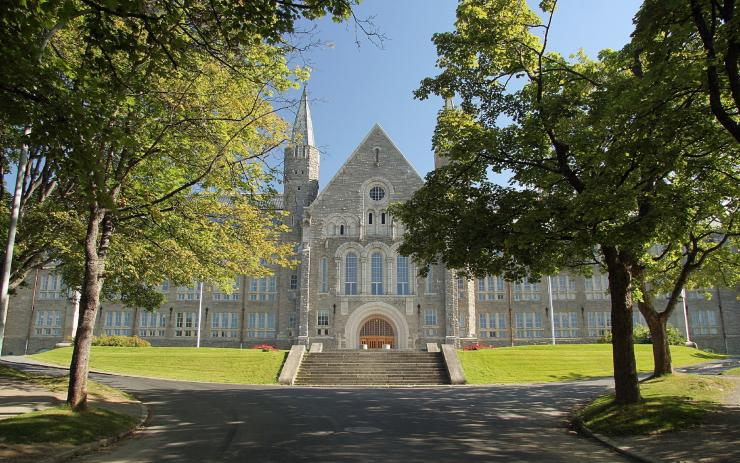
\includegraphics[width=1in]{picture/NTNU}
\end{wrapfigure}

I worked during this internship in the department of Electric Power Engineering at NTNU with other students from different universities from juin 3rd to August 25th 2015.
The Norwegian University of Science and Technology (Norwegian: Norges teknisk-naturvitenskapelige universitet, abbreviated NTNU) is a public research university located in the city of Trondheim, Norway. NTNU is the second largest of the eight universities in the country, and, as its name suggests, has the main national responsibility for higher education in engineering and technology. In addition to engineering and the natural and physical sciences, the university offers advanced degrees in other academic disciplines ranging from the social sciences, the arts, medicine, architecture and fine art.

\subsection{Project}

This project, working in collaboration with the Royal University of Bhutan is aimed at developing the design tools needed to build a prototype PV-microgrid at the College of Science and Technology in Bhutan. This project will be supporting this Micro grid by proposing a design tool that can identify the following:
- Optimal microgrid structure and composition
- Methods for simplifying the planning and resource-assessment phase
- Full year simulation of the system, with measurements on load, production, voltage and frequency
- 24 hours simulation in order to analyse in details the behaviour of the system
In this project a team had already doing a preliminary assessment that will be used as starting point.
This work is in collaboration with Engineers without Borders Norway and the Royal University of Bhutan.
A great part of our work is open source and available on line \url{<https://github.com/microgrid>}.

\subsection{Bhutan "the last Paradise on earth"}

\begin{wrapfigure}{l}{1in}
    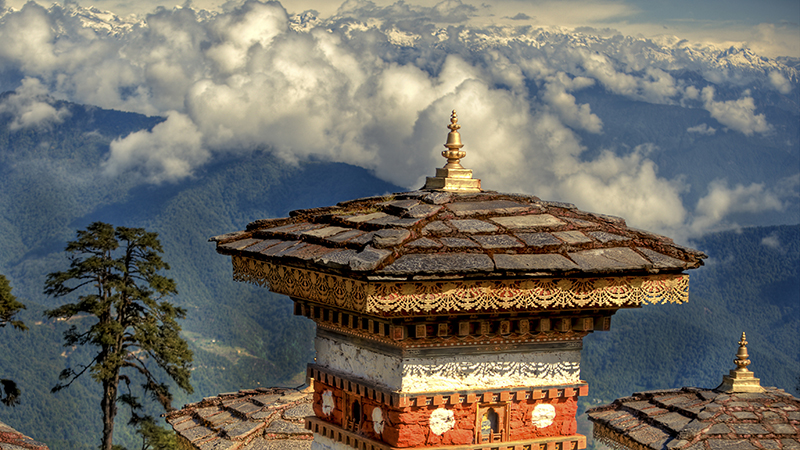
\includegraphics[width=1in]{picture/bhutan}
\end{wrapfigure}

The Kingdom of Bhutan \og Land of the Thunder Dragon\fg{} is a landlocked country in South Asia at the eastern end of the Himalayas.Bhutan is a constitutional monarchy with a unitary parliament and the last standing Buddhist Kingdom in the world.
National Happiness instead of a Gross Domestic product as a policy, thus having as one of their fundamental pillars the conservation of nature. Bhutan is considered to be one of the happiest countries in the world along with a great biodiversity. Therefore, unlike the rest of the world, economic growth is not a priority.
The Bhutanese government has recently enacted a Renewable Energy Policy. This is to ensure development in the area, so that the all inhabitants are given access to electricity through sustainable measures.  Additionally, the Carbon Neutrality Strategy launched by the government in 2012 makes Bhutan one of the few countries in remaining carbon-neutral. 
Due to the current national infrastructure, small off-grid PV-systems is a good alternative solution to accommodate this desire and ways for rapid implementation needs to be explored.
https://library.blogs.law.pace.edu/2014/12/02/bhutan-the-last-paradise-where-humans-and-environment-can-coexist/

\subsection{The Team}

%\begin{wrapfigure}{l}{1in}
%    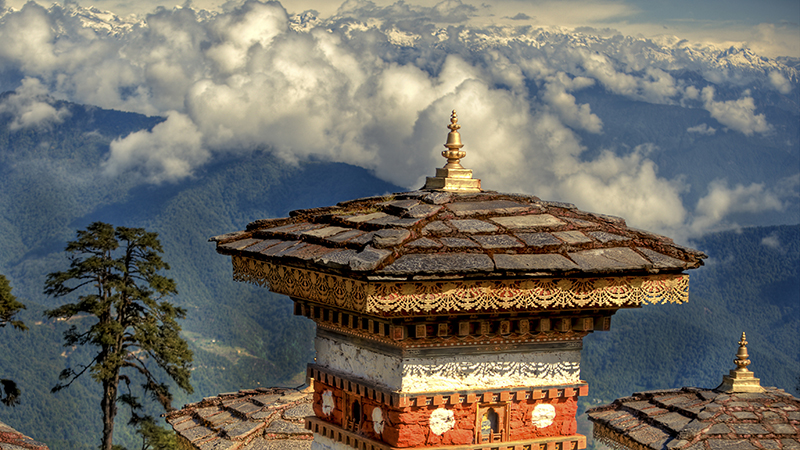
\includegraphics[width=1in]{picture/bhutan}
%\end{wrapfigure}

\subsubsection{Composition}

%\begin{wrapfigure}{l}{1in}
%    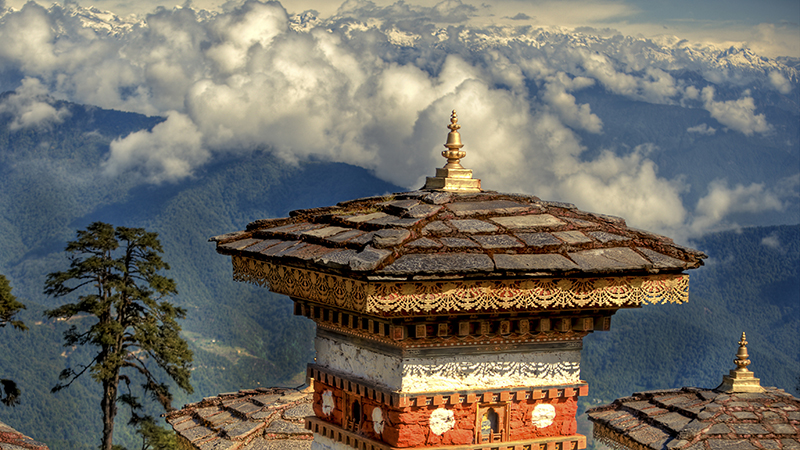
\includegraphics[width=1in]{picture/bhutan}
%\end{wrapfigure}

\subsubsection{Tasks}
\section{Methodology}

\subsection{Specification}

\subsubsection{Power source}

The source will be composed in the first time by PV panels since the country enjoys a good sunshine. In addition, a biomass generator should be used as backup power but this part will be implemented later.

\subsubsection{Insolation data analysis and projections}

In order to size and simulate the Microgrid, the first step was to get different data. Usually ground measurements are more reliable than satellite information but the lack of ground sensors in Bhutan involve in our case that we had to use the website \url{<https:https://eosweb.larc.nasa.gov/sse/>} which provides for free the insolation and the temperature. Therefore, these values are based on the year 2012 so we will have to take into account the evolution of the different parameters through the last 13 years due especially to the climate change.

\subsubsection{Data Acquisition}

We obtain first from the website the daily average insolation incident on a horizontal surface ($kWh/m^2/day$) per day for a full year (2012).
 From that point, we constituted a daily average insolation incident on a horizontal surface ($kWh/m^2/day$) for each month.
 

\subsubsection{Direct insolation data}
\subsubsection{Temperature data analysis and projections}
\subsubsection{Loads profile}

\subsection{State design}
\subsubsection{Generator power}
\subsubsection{Outage voltage}
\subsubsection{Load}

\subsection{State design}

\subsubsection{GitHub}


\end{document}


